%%%%%%%%%%%%%%%%%%%%%%%%%%%%%%%%%%%%%%%%%

% LaTeX Template for IAHR YPN Congress

%%%%%%%%%%%%%%%%%%%%%%%%%%%%%%%%%%%%%%%%%

%----------------------------------------------------------------------------------------
%	PACKAGES AND OTHER DOCUMENT CONFIGURATIONS
%----------------------------------------------------------------------------------------

\documentclass[landscape,a0paper,fontscale=0.285]{baposter} % Adjust the font scale/size here

\usepackage{graphicx} % Required for including images
\graphicspath{{figures/}} % Directory in which figures are stored

\usepackage{hyperref}
\hypersetup{colorlinks, citecolor=blue, filecolor=blue, linkcolor=blue, urlcolor=blue}

\usepackage{amsmath} % For typesetting math
\usepackage{amssymb} % Adds new symbols to be used in math mode
\usepackage[russian]{babel} % указать, что язык текста - русский
\usepackage{booktabs} % Top and bottom rules for tables
\usepackage{enumitem} % Used to reduce itemize/enumerate spacing
\usepackage{palatino} % Use the Palatino font
\usepackage[font=small,labelfont=bf]{caption} % Required for specifying captions to tables and figures
\usepackage{graphicx}
\usepackage{multicol} % Required for multiple columns
\setlength{\columnsep}{1.5em} % Slightly increase the space between columns
\setlength{\columnseprule}{0mm} % No horizontal rule between columns

\usepackage{tikz} % Required for flow chart
\usetikzlibrary{shapes,arrows} % Tikz libraries required for the flow chart in the template

\newcommand{\compresslist}{ % Define a command to reduce spacing within itemize/enumerate environments, this is used right after \begin{itemize} or \begin{enumerate}
\setlength{\itemsep}{1pt}
\setlength{\parskip}{0pt}
\setlength{\parsep}{0pt}
}

\definecolor{lightblue}{rgb}{0.145,0.6666,1} % Defines the color used for content box headers

\begin{document}

\begin{poster}
{
headerborder=closed, % Adds a border around the header of content boxes
colspacing=1em, % Column spacing
bgColorOne=white, % Background color for the gradient on the left side of the poster
bgColorTwo=white, % Background color for the gradient on the right side of the poster
borderColor=lightblue, % Border color
headerColorOne=black, % Background color for the header in the content boxes (left side)
headerColorTwo=lightblue, % Background color for the header in the content boxes (right side)
headerFontColor=white, % Text color for the header text in the content boxes
boxColorOne=white, % Background color of the content boxes
textborder=roundedleft, % Format of the border around content boxes, can be: none, bars, coils, triangles, rectangle, rounded, roundedsmall, roundedright or faded
eyecatcher=true, % Set to false for ignoring the left logo in the title and move the title left
headerheight=0.1\textheight, % Height of the header
headershape=roundedright, % Specify the rounded corner in the content box headers, can be: rectangle, small-rounded, roundedright, roundedleft or rounded
headerfont=\Large\bf\textsc, % Large, bold and sans serif font in the headers of content boxes
%textfont={\setlength{\parindent}{1.5em}}, % Uncomment for paragraph indentation
linewidth=2pt % Width of the border lines around content boxes
}
%----------------------------------------------------------------------------------------
%	TITLE SECTION 
%----------------------------------------------------------------------------------------
%
{\includegraphics[height=6em]{frkt_logo.png}} % First university/lab logo on the left
{\bf\textsc{Работа 4.5.2\\ Интерференция лазерного излучения}\vspace{0.5em}} % Poster title
{\textsc{Мария Шлапак, МФТИ }} % Author names and institution
{\includegraphics[height=6em]{logo.png}} % Second university/lab logo on the right

%----------------------------------------------------------------------------------------
%	ABSTRACT
%----------------------------------------------------------------------------------------

\headerbox{Введение}{name=abstract,column=0,row=0}{


\vspace{0.6em}

\textbf{Ключевые слова:} \em гелий-неоновый лазер, интерференция, когерентность, видность, излучение \em

\vspace{0.3em} % When there are two boxes, some whitespace may need to be added if the one on the right has more content
}

%----------------------------------------------------------------------------------------
%	INTRODUCTION
%----------------------------------------------------------------------------------------

\headerbox{Цель работы}{name=introduction,column=1,row=0,bottomaligned=abstract}{
Исследовать видность интерференционной картины излучения гелий-неонового лазера и определить длину когерентности излучения

}

%----------------------------------------------------------------------------------------
%	RESULTS 1
%----------------------------------------------------------------------------------------

\headerbox{Результаты эксперимента}{name=results,column=2,span=2,row=0}{
\small
\begin{enumerate}
    \item Зависимость $V$ от угла поворота $\beta$ поляроида П1 при нулевой разности хода\\
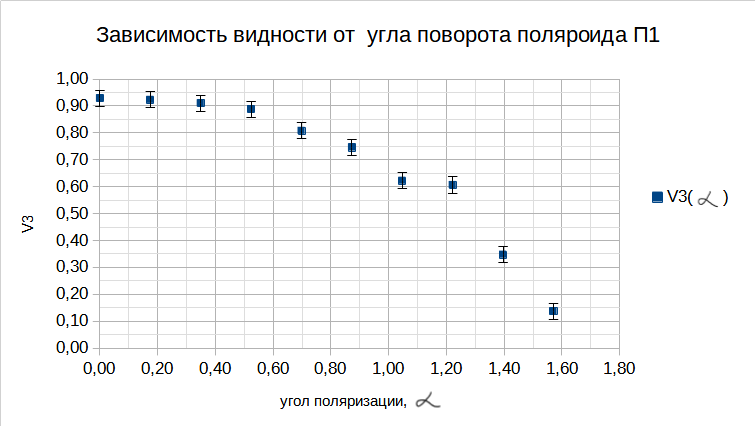
\includegraphics[width=5cm]{g1.png}
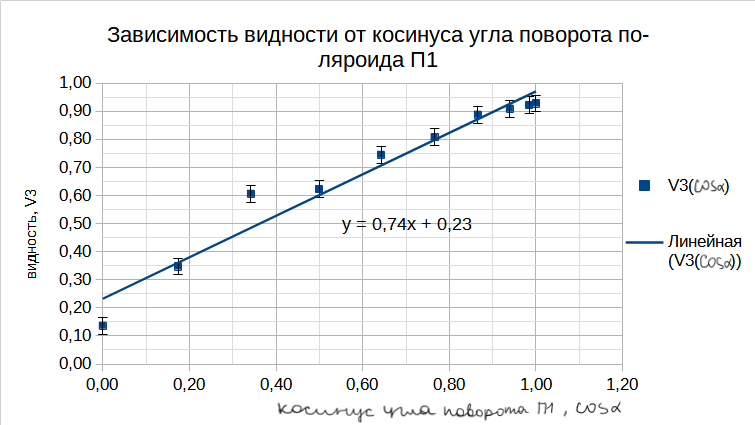
\includegraphics[width=5cm]{g2.png} 
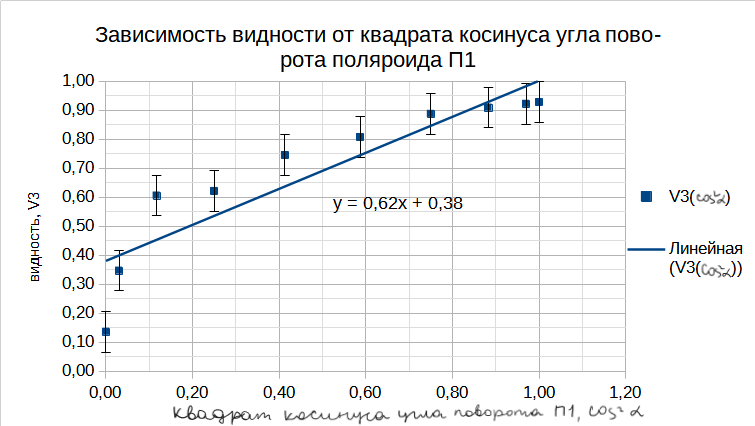
\includegraphics[width=5cm]{g3.png} \\
\textit{Рис.3. Зависимость V3 от угла поворота П1}\\
\item Зависимость $V$ от разности хода между пучками
\begin{multicols}[2]
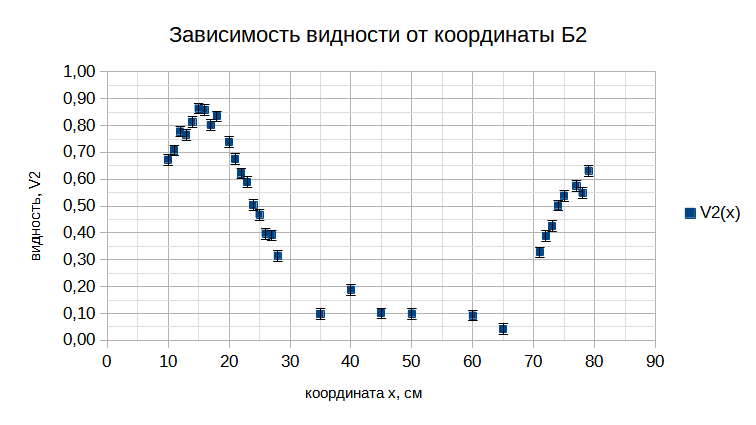
\includegraphics[width=6cm]{g4.png} \\
\textit{Рис.4. Зависимость V2 от координаты Б2}\\
\\
По полученному графику вычислим  $L$ и $\triangle \nu$ по формуле (1):\\
$L = \frac{2x}{2} = 62 \; L = (62 \pm 3) \; \textit{см}$\\
$\triangle \nu = \frac{c}{2L} \; \triangle \nu = (2,41 \pm 0,06)\cdot 10^8 \; \textit{Гц}$\\
Задержка $l_{1/2}$ на половине чатсоты главного максимума: $l_{1/2} \approx 11$ см\\
Диапазон чатсот, в котором происходит генерация продольных мод: $2\triangle F \approx 1,45\cdot 10^9 $ Гц\\
Число генерируемых лазером продольных мод: $N = 1 + \frac{2\triangle F}{\triangle \nu} \approx 7$\\
\end{multicols}


\end{enumerate}
}\\
%----------------------------------------------------------------------------------------
%	REFERENCES
%----------------------------------------------------------------------------------------

\headerbox{Используемая литература}{name=references,column=0,above=bottom}{
\textit{1. Общий курс физики. Оптика, Д.В.Сивухин}\\
\textit{2. Лабораторный практикум по общей физике. Оптика, А.В. Максимычев}\\
}

%----------------------------------------------------------------------------------------
%	FUTURE RESEARCH
%----------------------------------------------------------------------------------------

\headerbox{Другие статьи на эту тему}{name=futureresearch,column=1,span=2,aligned=references,above=bottom}{ % This block is as tall as the references block
\begin{description}\compresslist
\item[1]\url{https://faraday.physics.utoronto.ca/IYearLab/intdif.pdf}
\item[2]\url{https://iopscience.iop.org/article/10.1088/1361-6404/ac0877/pdf}
\end{description}
}

%----------------------------------------------------------------------------------------
%	CONTACT INFORMATION
%----------------------------------------------------------------------------------------

\headerbox{Contact Information}{name=contact,column=3,aligned=references,above=bottom}{ % This block is as tall as the references block

\begin{description}\compresslist
\item[Email]\url{shlapak.mv@phystech.edu}
\end{description}
}

%----------------------------------------------------------------------------------------
%	CONCLUSION
%----------------------------------------------------------------------------------------

\headerbox{Вывод}{name=conclusion,column=2,span=2,row=0,below=results,above=references}{

}

%----------------------------------------------------------------------------------------
%	MATERIALS AND METHODS
%----------------------------------------------------------------------------------------

\headerbox{Теоретические основы}{name=method,column=0,below=abstract,bottomaligned=conclusion}{ % This block's bottom aligns with the bottom of the conclusion block
\small
Разрешенные частоты и длины волн для лазера:
\begin{equation}
\frac{2\pi}{\lambda}2L = 2\pi m \; , L = m\lambda \;,
\nu_m = \frac{mc}{2L} \; , \traingle \nu_m  = \frac{c}{2L}
\label{eq:refname}
\end{equation}
Генерирующиеся лазером отдельные типы колебаний назвали \em модами \em.\\
Для оценки чёткости интерференционной картины в окрестности некоторой точки используют параметр видности:
\begin{equation}
V = \frac{I_{max} - I_{min}}{I_{max} + I_{min}}
\label{eq:refname}
\end{equation}
Человеческий глаз уверенно различает чередование светлых и тёмных интерференционных полос, если $V > 0,1$\\
Пусть в плоскости наблюдения интерферируют под небольшим углом две волны с амплитудами $A_m$ и $B_m$. Нетрудно догадаться, что видность выражается как
\begin{equation}
V_1 = \frac{2\sqrt{\delta}}{1 + \delta} \; , \delta = \frac{B^2_m}{A^2_m}
\label{eq:refname}
\end{equation}
Пусть теперь лазер генерирует одновременно несколько мод с одинаковой амплитудой, тогда:
\begin{equation}
V_2 = |\frac{1}{n}\frac{\sin \frac{\pi l}{2L}n}{\sin \frac{\pi l}{2L}}| \; , \textit{$l$ - разность путей между пучками}
\label{eq:refname}
\end{equation}
Если обе волны линейно поляризованы, а угол между плоскостями поляризаций равен $\beta$, то в выражениях для видности добавится множитель $V_3 = \cos \beta$. Если же направление поляризации хаотически меняется от $0$ до $\pi$, то $V_3 = \cos^2 \beta$. \\
Если имеют место все три фактора уменьшения видности, то результирующая видность:
\begin{equation}
V = V_1 \cdot V_2 \cdot V_3
\label{eq:refname}
\end{equation}
}

%----------------------------------------------------------------------------------------
%	RESULTS 2
%----------------------------------------------------------------------------------------

\headerbox{Экспериментальная установка}{name=results2,column=1,below=abstract,bottomaligned=conclusion}{ % This block's bottom aligns with the bottom of the conclusion block


\vspace{1em}
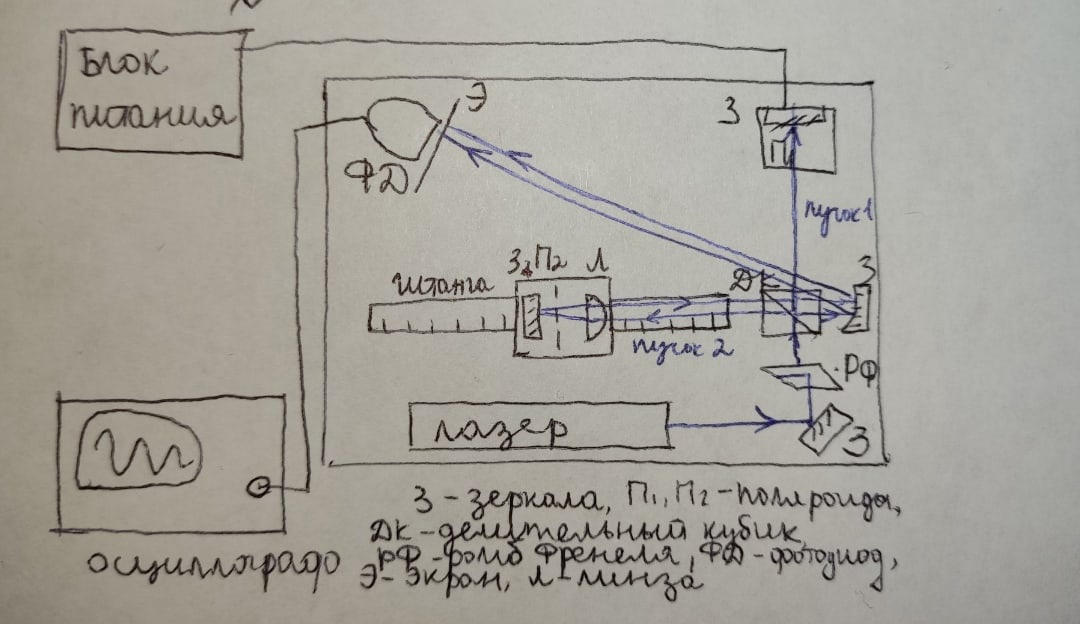
\includegraphics[width=7cm]{exp1.jpg}\\
\textit{Рис.1. Экспериментальная установка}\\
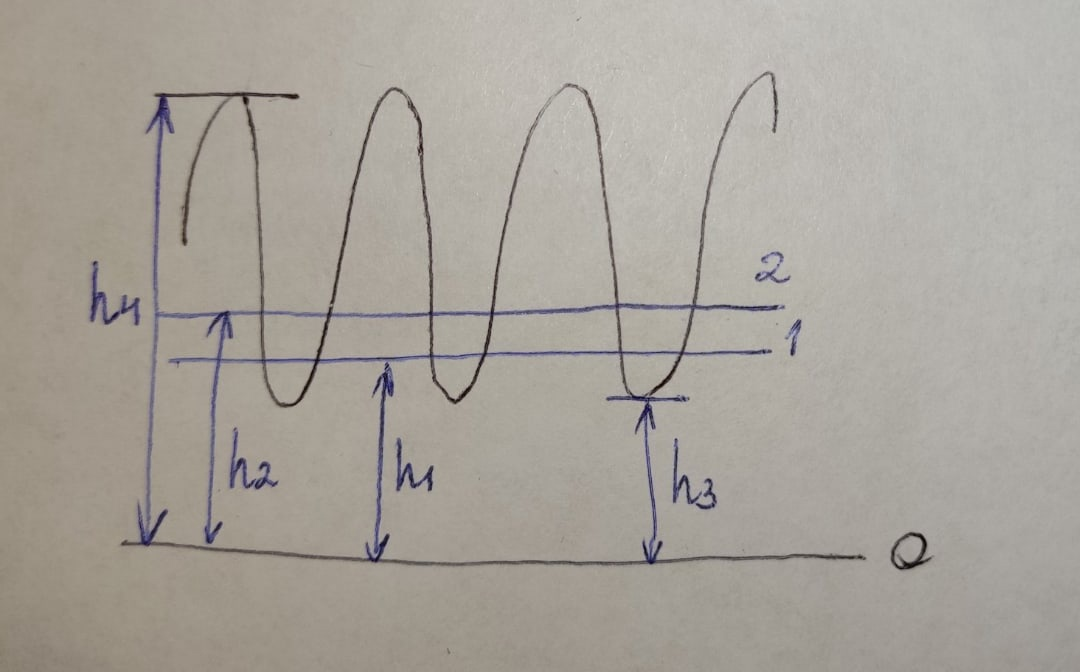
\includegraphics[width=7cm]{exp2.jpg}\\
\textit{Рис.2. Осциллограмма сигналов с фотодиода}\\
\begin{center}
    \textbf{Измерение видности}
\end{center}
Видность интерференционной картины считается по формуле: 
$V = \frac{h_4 - h_3}{h_4 + h_3}$


Для угла между плоскостями поляризации $\beta = 0$: $V_2(l) = \frac{V}{V_1}$\\
или при $l = 0$ для известного $\beta$: $V_3 = \frac{V}{V_1}$

}

%----------------------------------------------------------------------------------------

\end{poster}

\end{document}